\documentclass[rep.tex]{subfiles}
\begin{document}

\chapter{Zadanie 2}
\label{zad2}
\section{Treść}
Dana jest powietrzna linia współosiowa o średnicach przewodów $\mathrm{a} = 7~mm$ i $\mathrm{b} = 3.04~mm$, patrz rys.~\ref{fig:zad2:coax}.
O ile należy przesunąć przewód wewnętrzny względem przewodu zewnętrznego ($\mathrm{c} = ?$) aby jej impedancja charakterystyczna zmieniła się o $5~\Omega$.

\begin{figure}[!htbp]
  \centering
  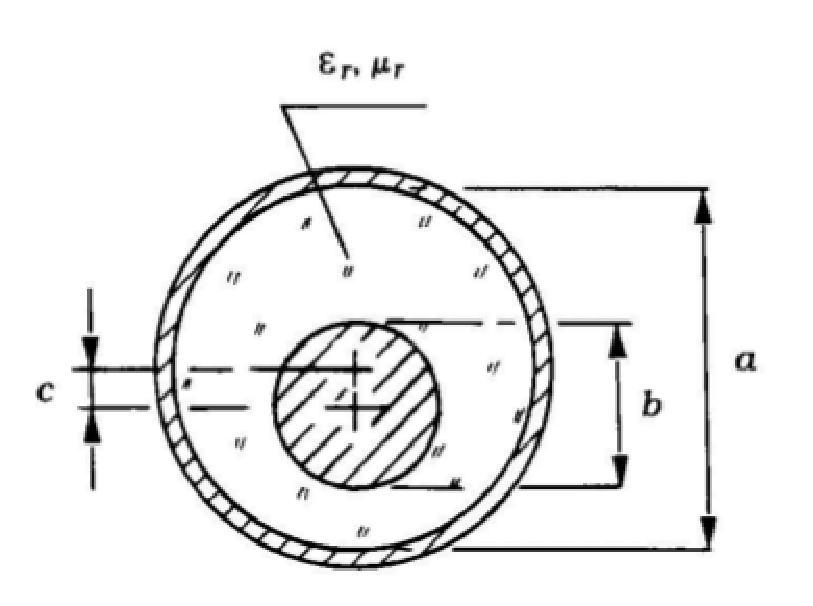
\includegraphics[scale=0.5]{fig/zad2/coax}
  \caption{Linie z przesuniętym przewodem wewnętrznym}
  \label{fig:zad2:coax}
\end{figure}

\section{Rozwiązanie}
Impedancja linii ekscentrycznej jest określona wzorem:
\begin{align}
  Z_0(x) &= 59.952 \sqrt{\frac{\mu_r}{\epsilon_r}}\ln\big(x + \sqrt{x^2 - 1}\big) \\
  x      &= \frac{1}{2a}\bigg(b + \frac{a^2 - 4c^2}{b}\bigg) \label{eqn:zad2:x}
\end{align}
Dla $\mathrm{c} = 0$  mamy:
\begin{equation}
  Z_0(x)\Big\arrowvert_{c=0} = 59.952 \sqrt{\frac{\mu_r}{\epsilon_r}}\ln\frac{a}{b} \label{eqn:zad2:z}
\end{equation}
Jest to zależność przybliżona.
Dokładny wzór na impedancje linii współosiowej ma postać:
\begin{equation}
  Z_0 = \frac{1}{2\pi} \sqrt{\frac{\mu}{\epsilon}}\ln\frac{a}{b}
\end{equation}
Porównując podane wyżej zależności dla $\mathrm{c} = 0$ mamy:\\
\begin{tabular}{l @{ : } l}
wzór dokładny    & 50.0085378279 \\
wzór przybliżony & 50.0031234918 \\
\end{tabular}\\
co daję błąd równy 0.01\%.

Zadanie można rozwiązać na 2 sposobu: analitycznie i numerycznie.
kolejne zadania będzie można rozwiązać już tylko numerycznie więc porównując rozwiązanie analityczne i numeryczne zadania~\ref{zad2} można przetestować zaprogramowaną metodę newtona.

\subsection{Rozwiązanie analityczne}
Równanie z jakie należy rozwiązać to 
\begin{align}
  \underbrace{59.952 \sqrt{\frac{\mu_r}{\epsilon_r}}}_k\ln\big(x + \sqrt{x^2 - 1}\big) &= \underbrace{\frac{1}{2\pi} \sqrt{\frac{\mu}{\epsilon}}\ln\frac{a}{b} - 5}_d \\
  \ln\big(x + \sqrt{x^2 - 1}\big) &= \frac{d}{k} \label{eqn:zad2:anal}
\end{align}
Kluczowe jest spostrzeżenie, że $\operatorname{arch}\,x = \ln\big(x + \sqrt{x^2 - 1}\big)$.
Biorąc cosinus hiperboliczny obu stron równania mamy
\begin{align}
  \operatorname{ch}\,(\operatorname{arch}\,(x)) &= \operatorname{ch}\,\frac{d}{k} \\
  x &= \frac{1}{2}\big(e^{\frac{d}{k}}+e^{-\frac{d}{k}}\big)
\end{align}
Otrzymane $x$ należy podstawić do wzoru~\ref{eqn:zad2:x}.
Po kilku przekształceniach otrzymuję się zależność:
\begin{align}
  c = \sqrt{\bigg(a^2 - ab2\operatorname{ch}\,\frac{d}{k} + b^2\bigg)\bigg/4}
\end{align}
Podstawiając dane z treści zadania otrzymuję się przesunięcie~$c = 0.882307292061 mm$.

\subsection{Rozwiązanie numeryczne}
W celu znalezienia wymaganego przesunięcia,
należy znaleźć wartość $\mathrm{x}$ przy którym impedancja spełnia warunek:
\begin{align}
  Z_0(x)\Big\arrowvert_{c=?} & = Z_0(x)\Big\arrowvert_{c=0} - 5 \\
  Z_0(x)\Big\arrowvert_{c=?} & - Z_0(x)\Big\arrowvert_{c=0} + 5 = 0
\end{align}
a następnie znając $x$ wyznaczyć $c$.
Oczywiście stosując rozwiązania numeryczne nie trzeba stosować się do kolejności wyznaczania (tzn. najpierw $x$ a potem $c$).
Dysponując funkcjami wyznaczającymi wartość impedancji można odnaleźć od razu $c$.

Wynik rozwiązany za pomocą zaprogramowanego algorytmu Newtona-Raphsona wynosi:
\begin{align}
  c_{numeryczne}  &= 0.882307221883 mm \nonumber \\
  c_{analityczne} &= 0.882307292061 mm \nonumber
\end{align}
różnica pomiędzy wynikami wynosi~$8.12217580519e-11$,
co jest zgodne z przyjętym kryterium zatrzymania pracy algorytmu na poziomie~$1e-10$.

\end{document}
